\chapter{Describing a layered architecture in Haskell} \label{chap:archCombs}

\bc
Puntjes

doc/pres/gest/upd or high/low/ehigh/elow?

opmerking: architecture is program, sometimes good, sometimes bad. ???? komt dit uit Medv&Taylor?

mention that it's not Haskell98

params for step Step ... a b = a->b or Step a b ... = a->b


Order of hor and vert is not ideal.  
f hor vert = (vert, hor) is most logical, but looks strange
f vert hor = (vert, hor) looks better but doesn't make it logical to parameterize f with its hor arg
f hor vert = (hor, vert) is chosen in thesis. result is a bit weird because vert is more logical on the left


Keertje uitzoeken of existential types dit allemaal mooier kunnen maken.
\ec



In this chapter we set of Haskell combinators for describing the layered architecture of Proxima, which was described in Chapter~\ref{chap:proxArch} and specified in the previous Chapter. Although designed with a layered editor in mind, the method is applicable to layered architectures in general. It has been successfully used not only for the implementation of the Proxima prototype, but also for a system that provides web-interfaces to databases. 

Haskell is a functional language with strong support for abstraction. Describing an architecture in an actual programming language not only makes it possible to verify the types of the components of the architecture, but also provides a framework for implementing the system that is described by the architecture. Because the architecture description in Haskell is a program in itself, the system can be instantiated by providing implementations for each of the components.

In their survey of architecture description languages (ADLs)~\cite{medvidovic00ADLs}, Medvidovic and Taylor identify three essential components of an architecture description: a description of the (interface of the) components, a description of the connectors, and a description of the architectural configuration. They claim that the focus on {\em conceptual} architecture and explicit treatment of connectors as first-class entities differentiate ADL's from, amongst others, programming languages. However, Higher-order typed (HOT) functional programming languages, such as Haskell, Clean~\cite{plasmeijer01clean}, and ML~\cite{milner97ML} offer possibilies for describing the main components of an architecture, and treating all of these components as first-class entities. Furthermore, by using abstraction, the description of the architecture can be focused on the conceptual architecture, while the details are left to the actual components.

As argued by Hudak~\cite{hudak98DSLs}, higher-order typed functional languages offer excellent possibilities for embedding domain-specific languages. Embedding a domain-specific language facilitates reuse of syntax, semantics, implementation code, software tools, as well as look-and-feel. We give a DSEL in Haskell for describing layered editor architectures. We use records that contain functions to describe the components of the architecture. The connectors are combinators, and the configurations are programs (functions) that consist of combinators and components. 

\bc
The requirements for a DSEL for describing architectures are slightly different from the requirements for more familiar applications of DSELs, such as parsers, pretty printers, etc. The latter are used to write programs that contain many applications of the combinators and that are usually subject to frequent change. An architecture description, on the other hand, will typically be a small and rather static entity, because changes to the architecture involve changes to many components of the system. \note{is dit wel zo? misschien is concise syntax toch wel zo handig.} As a consequence, a concise syntax for combinator expressions is not of the highest importance.
\ec

\bc Another difference concerns the efficiency of the combinators.\ec 

Often, a program that makes use of a DSEL, contains many applications of the combinators, and hence the evaluation of the combinators forms a substantial part of the running time. Consider, for example, parsers or pretty printers. In contrast, the combinators in an architecture description are just the glue that connects the main components of the system. Most of the running time of the system can be expected to be taken up by the components and not by the combinators. Therefore, efficiency of the combinators is not a major concern. Wrapping and unwrapping a few values in the combinators is not a problem if it improves the transparency of the architecture.

In this chapter we give four implementation models for layered architectures. First, we introduce a simple example layered editor architecture and explore how its main components can be modeled in Haskell. Then we proceed to connect the components. In Section~\ref{sect:simple} the connection is straightforward, with little abstraction. This is used in Section~\ref{sect:ncp} as a basis to develop a more abstract combinator implementation that uses nested pairs. In Section~\ref{sect:hidden}, we present another set of combinators, which employ a form of state hiding to improve on the previous set. Section~\ref{sect:lib} develops a small generic library for building the architecture-specific combinators of Section~\ref{sect:hidden}. Finally, in Section~\ref{sect:proxima}, we show how the architecture combinators are used to describe (and implement) the architecture of  the Proxima editor.%Section~\ref{sect:haskellconclusions} presents the conclusions.



%																
%																
%																
\section{A simple editor}


We introduce a simple layered architecture for a presentation-oriented editor, which is used in the next sections to explain the architecture description methods. Although the architecture is simple, it contains the essential features of the Proxima architecture discussed in Chapter~\ref{chap:proxArch}. In Section~\ref{sect:proxima} we will show how the architecture combinators are used in the implementation of Proxima.

Figure~\ref{simpleeditprocess} depicts the editing process for our simple editor. The editor keeps track of a document ($doc$), which is mapped onto a presentation ($pres$). The presentation process is split into $n$ components: $\present_1 \dots \present_n$. At the bottom of the figure, the presentation is shown to a user, who provides an edit gesture ($gest$) in response. The edit gesture is then mapped onto a document update ($upd$) by $\interpret_n \dots \interpret_1$, after which it is performed on the document.

%\bl
%\o ref to informal spec
%\o not incremental. 
%\o doc is kept at the top
%\el
%View is similar to Chapter~\ref{chap:proxArch} . 

A layer consists of a pair of $\present_i$ and $\interpret_i$ functions, which we also refer to as {\em layer functions}. Besides the vertical data flow for presentation and interpretation, we may also have horizontal data flow that stays within the layer. Horizontal data flow concerns results from a layer function that are passed to a layer function it the same layer, possibly in a next edit step.

Figure~\ref{simplesinglelayer} shows the data flow for a single layer with two examples of horizontal data flow. The $mapping$ result of $\present$ is passed to $\interpret$ and represents information about the presentation mapping. Furthermore, a $state$ parameter is passed to $\present$ as well as $\interpret$, and may be updated by $\interpret$. Note that the $state$ parameter of $\present$ is the result of $\interpret$ in the previous edit step. Because of the sequential nature of the edit steps, we only consider horizontal data flow that goes from left to right.

The editor can only support direct interpretation (see Section~\ref{sect:intrProcess}) because the value of the data level is not available at the interpretation step. This is not a realistic situation, but for our example it does not matter. The Proxima layer that will be explained in Section~\ref{sect:proxima} also supports indirect interpretation, because it keeps the value of the data level in the horizontal data flow.

%A more realistic example of horizontal data flow is the value of a data level.  is values of the levels, so vertical are just edit ops. This is %what is done in Proxima (see Section~\ref{sect:proxima})
%We can find an example of horizontal dataflow in an incremental editor: the values for the data levels .  



\bc
If we look at the figure, we see that there are values that go from left to right, and values that go either up or down. The values that go in horizontal direction are computed by the functions in the corresponding layer, although not necessarily in the same edit cycle. The vertical direction parameter for a layer function, on the other hand, is the result of that function in a neighboring layer (i.e.\ a {\em present} layer function gets its vertical parameter from another {\em present} function, and an {\em interpret} layer function gets it from another {\em interpret} function). When composing layers, the vertical results from one layer are passed as parameters to the next layer. The outermost vertical parameter is the parameter to the combined layer, and the outermost vertical result is the result of the combined layer. 
\ec
\bc
******* Extra state verhaal nog even bekijken  niet 2 x ref formalSpec
\head{\bf A single layer}

Figure~\ref{simplesinglelayer} shows the data flow for a single layer. It is somewhat more complex than Figure~\ref{simplelayers} \note{figure: dotted line between present and interpret}, because not all horizontal parameters to $interpret$ are results of $present$ \note{i.e.\ wg?} (i.e.\ $state$ is not a result of $present$). The data flow is a simplification of the data flow of the layered editor with extra state from ****Chapter~\ref{chap:formalSpec}. $present$ maps a high level data structure $doc$ to a low level data structure $pres$. The $state$ parameter contains state that is local to the layer, as described in ****Chapter~\ref{chap:formalSpec} \note{change to internal ref}. The $interpret$ function works in the opposite direction of $present$ and maps an edit operation ($gest$) on the $pres$ data structure to an edit operation ($upd$) on the $doc$ data structure. Besides $pres$, $present$ also returns a value $mapping$. It is used to encode information that is required by $interpret$ in order to map $gest$ to $upd$. An example of such information is a table of pointing information, that relates objects in $pres$ to their origin in $doc$. Because $gest$ may be an edit operation on the extra state, $interpret$ also has $state$ as a parameter. In that case, $state'$ is the result of performing the update on the extra state. In any other case, $state'$ is equal to $state$. 
\ec

\begin{figure}
\begin{small}
\begin{center}
\begin{center}
\begin{minipage}[b]{\textwidth}
\begin{scriptsize}
\xymatrix@=0.5cm{
\ar@{.>}[r] & \dataa{$doc$}\ar[d] & \dataa{$upd$} \ar@{.>}[r]& \dataa{$doc$}\ar[d] & \dataa{$upd$} \ar@{.>}[r]& \\
 & \component{$\present_1$}  \ar@{.>}[d]	& \component{$\interpret_1$} \ar[u]    & \component{$\present_1$}  \ar@{.>}[d]& \component{$\interpret_1$} \ar[u]    \\ 
& \component{$\present_n$} \ar[d]      	& \component{$\present_n$} \ar@{.>}[u] & \component{$\present_n$} \ar[d]      & \component{$\present_n$} \ar@{.>}[u] \\ 
 & \dataa{$pres$} \ar@{.>}[r] &  \dataa{$gest$}\ar[u] & \dataa{$pres$} \ar@{.>}[r]&  \dataa{$gest$}\ar[u] \\
% \save"2,2"."3,3"*!=<6.105em,13ex>[F.]\frm{}\restore 
 \save"2,2"."3,3"*!=<12.1em,13ex>[F]\frm{}\restore 
% \save"2,4"."3,4"*!=<6.105em,13ex>[F.]\frm{}\restore
  \save"2,4"."3,5"*!=<12.1em,13ex>[F]\frm{}\restore 
}
\end{scriptsize}
\end{minipage}
\end{center}\caption{Two cycles in the editing process. (draft)}\label{simpleeditprocess} 
\end{center}
\end{small}
\end{figure}



\begin{figure}
\begin{small}
\begin{center}
\begin{center}
\begin{minipage}[b]{\textwidth}
\begin{scriptsize}
\xymatrix @R=1pc{
& & \dataa{$doc$}\ar[d] & & & \dataa{$upd$} & \\
\dataa{$state$}\ar[rr] \ar `r[rd] `[rr] `[rrrr] `[rrrr] [rrrrr] & & \dimcomponent{5em}{2ex}{\present} \ar[ddd] \ar[r] &
     \dataa{$mapping$}\ar[rr] & & \dimcomponent{6em}{2ex}{\interpret} \ar[u] \ar[r] & \dataa{$state$} \\
& & & & & \hspace{3.5em} &  \\
& & & & & \hspace{3.5em} &  \\
& & \dataa{$pres$} & & & \dataa{$gest$}\ar[uuu] & 
 \save {"2,2"."3,6"* +<2em,3em>[F] \frm{}}\restore
}
\end{scriptsize}
\end{minipage}
\end{center}\caption{A single layer.  (draft)}\label{simplesinglelayer} 
\end{center}
\end{small}
\end{figure}

\bc \head{\bf The layers}

Figure~\ref{simplelayers} \note{figure: dotted line between present and interpret} shows a more detailed view of a single edit cycle. For now, we focus on the presentation and interpretation phases (phase 1 and phase 4). Both the presentation and the interpretation functions (we will call them {\em present} and {\em interpret}) are compositions of a number of subfunctions, similar to the layered editor in Chapter~\ref{chap:formalSpec}. The presentation of a document is computed via a number of intermediate data structures that are increasingly concrete, and the edit operation on the document is computed via edit operations on the same intermediate data structures. Therefore, the subfunctions of {\em present} and {\em interpret} are grouped pairwise in horizontal layers. Another reason for grouping the subfunctions is that each subfunction in a layer has some parameters that are the result of the subfunction immediately to the left of it. We will refer to the subfunctions as {\em layer functions}. \ec


%The main loop of the simple editor consists of the following 5 phases: 
% 
% \begin{enumerate}
% \item Compute a rendering, or {\it presentation}, of the document  (presentation phase)
% \item Show the presentation to the user
% \item Receive an edit gesture from the user
% \item Interpret the edit gesture as a document update (interpretation phase)
% \item Compute the updated document
% \end{enumerate}



\bc
Figure~\ref{simpleeditprocess} contains a schematic representation of the editing process. Each of the boxes represents one complete edit cycle. The emphasis in the figure is put on the presentation and interpretation phases (phases 1 and 4). Phases 2 and 3 are represented by the dotted arrows at the bottom of the figure, and phase 5 is represented by the dotted arrows at the top.
\ec



%																
%																
%																
\section{A layer in Haskell} \label{sect:layerInHaskell}

In the following sections, we explore the possibilities of implementing the layered architecture from the previous section in the functional language Haskell. The use of a typed programming language for describing an architecture ensures that the types of all components are correct. Furthermore, because the architecture description language is equal to the implementation language, the architecture description is an executable framework for the system being described. Thus, we eliminate the extra step of translating the architecture description to a program, which is a possibe source for errors.


There are two aspects to modeling a layered architecture in Haskell: the building blocks, which are the layer functions, and the connections between the building blocks. In the next sections, we present three methods for modeling the connections, but first we focus on the layer functions. 

A layer function takes  horizontal as well as vertical arguments and returns both  horizontal and vertical results. To make the difference between horizontal and vertical data explicit, we introduce a type synonym for layer functions.

\bc single vertical result, tupled with one ore more horizontal results .In order to clearly distinguish between horizontal and vertical parameters, we write the type of a layer function in the following form: \p{horArg -> vertArg -> (vertRes, horRes)}. Thus, we see that a layer function takes one ore more horizontal arguments, a single vertical argument, and returns a single vertical result, tupled with one ore more horizontal results. We introduce a type synonym for layer functions of this type. \ec

%Maybe the current order does make sense. The horizontal args typically include
% sheets which are constant and should be among the first parameters. The 
%horizontal result is put second, because the   vertical result is what matters.
% The horizontal result is just necessary to compute a following vertical result.

%code from Haskell/DPPClass_Lib.hs
\begin{small}
\begin{verbatim}
type LayerFunction horArg vertArg horRes vertRes =
       horArg -> vertArg -> (horRes, vertRes)
\end{verbatim}
\end{small}

We model a layer with a record that contains the layer functions. For the example editor, we have the two layer functions: \p{present} and \p{interpret}. The types of the layer functions follow directly from Figure~\ref{simplesinglelayer}.  If we would put these functions directly in a record, we would get:

\bc The names of the type and selector functions contain an apostrophe (\p{'}) because we also introduce a slightly different type \p{Simple}, which will be used in most of the rest of this paper. \note{overal Simple gebruiken?} \ec

%code from Haskell/Layers.hs
\begin{small}
\begin{verbatim}
data Simple state mapping doc pres gest upd =
       Simple { present   :: LayerFunction state doc mapping pres
              , interpret :: LayerFunction (mapping, state) gest state upd
              }
\end{verbatim}
\end{small}


\bc ** beetje overbodig
Strictly speaking, \p{Simple} is not a type but rather a type constructor, but since it is inconvenient to have to supply the type parameters every time the type is mentioned, we will denote the type with its constructor in the remainder of this text. More formally, when refering to a type \p{t}, where \p{t} is a type constructor with $n$ parameters, we mean the type \p{t a$_1$ \dots ~a$_n$} for fresh type variables \p{a$_i$}.
\ec
However, this is not entirely what we want. To simplify the horizontal connection between layer functions, we prefer a normalized data type in which the horizontal result type (\p{horRes}) of a layer function matches the horizontal argument type (\p{horArg}) of the next layer function. For our example, this implies that the horizontal result of \p{present} has the same type as the horizontal argument of \p{interpret} and vice versa (since the result of \p{interpret} is the argument of \p{present} in the next edit cycle). Figure~\ref{wrapped} shows the data flow for the layer functions in the normalized type \p{Simple}. Because the conversion to a normalized type is straightforward, we do not show it here. The definition of the normalized \p{Simple} is:

\begin{small}
\begin{verbatim}
data Simple state mapping doc pres gest upd =
       Simple { present ::   LayerFunction state doc (mapping, state) pres
              , interpret :: LayerFunction (mapping, state) gest state upd
              }
\end{verbatim}
\end{small}


Note that the field names in the record (\p{present}, \p{interpret}) are also the names of the field selection functions. Thus, for a layer \p{layer0 :: Simple} we denote the presentation function by \p{present layer0}. 

%The \p{Simple'} type is parameterized with all the types that appear in the signatures of the layer functions.

\bc
Only in the next section, we use the type \p{Simple'}. Afterwards, \p{Simple} is used. Because conversions between the two types are trivial, we will not give them. The reason why we give \p{Simple'} at all is that it is the more appropriate type from the component programmer's view. It contains exactly the function types we expect the components to have, whereas in \p{Simple}, present returns the \p{state} parameter, which is done only to make connecting easier.
\ec

\bc
Now that the building blocks have been established, we need a way to connect them. We show three connection methods. First, we explicitly connect all parameters and results by hand, which is a working, but not very transparent, solution. Subsequently, we introduce two more elegant and abstract methods. These methods are specific to the \p{Simple'} and \p{Simple} data types, but from the last method we derive a small library that can be used for layers with an arbitrary number of layer functions. 
\ec

\begin{figure}
\begin{small}
\begin{center}
\begin{center}
\begin{minipage}[b]{\textwidth}
\begin{scriptsize}
\xymatrix@=0.6cm{
 & \dataa{$doc$}\ar[d]                    & & & \dataa{$upd$} & \\
 \dataa{$state$}\ar[r]                    & \dimcomponent{5em}{2ex}{present} \ar[dd] \ar `r[d] `[dr] [dr] \ar[r] &
     \dataa{$mapping$}\ar@{.>}[r] & \dataa{$mapping$} \ar[r] & \dimcomponent{6em}{2ex}{interpret} \ar[u] \ar[r] & \dataa{$state$} \\
 & & \dataa{$state$}\ar@{.>}[r] & \dataa{$state$} \ar `r[u] `[ru] [ru] & \hspace{3.5em} &  \\
 & \dataa{$pres$}                          & & & \dataa{$gest$}\ar[uu] & 
 \save"2,2"."3,5"*+<2em>[F.]\frm{}\restore 
}
\end{scriptsize}
\end{minipage}
\end{center}\caption{Data flow in a normalized layer. (draft)}\label{wrapped} 
\end{center}
\end{small}
\end{figure}


%																
%																
%																
\section{Method 1: Explicitly connecting the components} \label{sect:simple}

Now that the layers have been modeled, we need to realize the data flow by connecting the layer functions. The document must be fed into the layers at the top, yielding the presentation at the bottom, and similarly, the edit gesture must be fed into the bottom layer, yielding the document update. \bc The layers are records that contain functions, so  \ec The most straightforward way of tying everything together is to explicitly write the selection and application of each of the functions in each of the layers. 

We give an example edit loop that explicitly connects three layers: \p{layer0}, \p{layer1}, and \p{layer2} of type \p{Simple}. The data flow between the layer functions is shown in Figure~\ref{explicit}. The corresponding Haskell code for the edit loop is:


\begin{figure}
\begin{small}
\begin{center}
\begin{center}
\begin{minipage}[b]{\textwidth}
\begin{scriptsize}
\xymatrix@=0.6cm{
 & \dataa{{\tt doc}} \ar[d] & & \dataa{{\tt update}} & \\
 \dataa{{\tt state0}}\ar[r]  & \dimcomponent{5em}{2ex}{{\tt present}} \ar[dd] \ar `r[d] `[dr] [dr] \ar[r] &
     \dataa{{\tt mapping0}} \ar[r] & \dimcomponent{6em}{2ex}{{\tt interpret}} \ar[u] \ar[r] & \dataa{{\tt state0'}} \\
 & & \dataa{{\tt state0}} \ar `r[u] `[ru] [ru] & \hspace{3.5em} &  \\
 & \dataa{{\tt pres1}} \ar[d] & & \dataa{{\tt gest1}}\ar[uu] & \\
 \dataa{{\tt state1}}\ar[r]  & \dimcomponent{5em}{2ex}{{\tt present}} \ar[dd] \ar `r[d] `[dr] [dr] \ar[r] &
     \dataa{{\tt mapping1}} \ar[r] & \dimcomponent{6em}{2ex}{{\tt interpret}} \ar[u] \ar[r] & \dataa{{\tt state1'}} \\
 & & \dataa{{\tt state1}} \ar `r[u] `[ru] [ru] & \hspace{3.5em} &  \\
 & \dataa{{\tt pres2}} \ar[d] & & \dataa{{\tt gest2}}\ar[uu] & \\
 \dataa{{\tt state2}}\ar[r]  & \dimcomponent{5em}{2ex}{{\tt present}} \ar[dd] \ar `r[d] `[dr] [dr] \ar[r] &
     \dataa{{\tt mapping2}} \ar[r] & \dimcomponent{6em}{2ex}{{\tt interpret}} \ar[u] \ar[r] & \dataa{{\tt state2'}} \\
 & & \dataa{{\tt state2}} \ar `r[u] `[ru] [ru] & \hspace{3.5em} &  \\
 & \dataa{{\tt pres3}} & & \dataa{{\tt gest3}}\ar[uu] & 
\save"2,2"."3,4"*+<2em>[F.]\frm{}\restore 
\save"5,2"."6,4"*+<2em>[F.]\frm{}\restore 
\save"8,2"."9,4"*+<2em>[F.]\frm{}\restore 
}
\end{scriptsize}
\end{minipage}
\end{center}\caption{Data flow in and between layers. (draft)} \label{explicit} 
\end{center}
\end{small}
\end{figure}

%code from Haskell/Explicit.hs
\begin{small}
\begin{verbatim}
editLoop (layer0, layer1, layer2) states doc = loop states doc
 where loop (state0, state1, state2) doc = 
        do { -- Presentation process:
             let ((mapping0,state0'), pres1) = (present layer0) state0 doc
           ; let ((mapping1,state1'), pres2) = (present layer1) state1 pres1
           ; let ((mapping2,state2'), pres3) = (present layer2) state2 pres2

           ; showRendering pres3
           ; gest3 <- getGesture
 
             -- Interpretation process:
           ; let (state2'', gest2)  = (interpret layer2) (mapping2, state2') gest3
           ; let (state1'', gest1)  = (interpret layer1) (mapping1, state1') gest2
           ; let (state0'', update) = (interpret layer0) (mapping0, state0') gest1
       
           ; let doc' = updateDocument update doc
           ; loop (state0'', state1'', state2'') doc'
           }
\end{verbatim}
\end{small}

%\note{Horrible type sigs due to lots of variables}

%The five phases of the simple edit cycle as presented in the previous section are directly visible in the code. 
The redundant parentheses in the applications of \p{present} and \p{interpret} are used to stress that these functions are selector functions. The functions \p{showPresentation}, \p{getGesture}, and \p{updateDocument} are left unspecified, because we focus on the connection of the layer functions. 

The following function \p{main} calls \p{editLoop} with the correct parameters.

%code from Haskell/Explicit.hs
\begin{small}
\begin{verbatim}
main layer0 layer1 layer2 = 
 do { states <- initStates
    ; doc <- initDoc 
    ; editLoop (layer0, layer1, layer2) states doc
    }
\end{verbatim}
\end{small}

The functions \p{initStates} and \p{initDoc} provide the initial values for \p{states} and \p{doc}, and are left unspecified. The layers of the editor are arguments of the \p{main} function. An editor can now be instantiated by applying the function \p{main} to three \p{Simple} values that implement the different layers. The type system verifies that the implemented layer functions have the correct type signatures.

A disadvantage of the implementation of the edit loop sketched in this section is that the patterns of the data flow are not very transparent. The fact that the mapping parameters are horizontal parameters and that the presentation is a vertical parameter is not immediately clear from the program code. Moreover, explicitly encoding the standard patterns for upward and downward vertical parameters, increases the chance of errors. Finally, the number of layers is hard coded in the implementation. If the system is extended with an extra layer, variables have to be renamed. If each type appearing in the layers is distinct, the type checker catches mistakes but if some parameters or results have the same type, the type checker will not detect a problem when, for example, two such equally typed variables are swapped. 

%We will therefore try to find a more abstract way of connecting the layers.


%																
%																
%																
\section{Method 2: Nested pairs}\label{sect:ncp}

\begin{figure}
\begin{scriptsize}
\begin{center}
\begin{center}
\begin{minipage}[b]{\textwidth}
\xymatrix@=0.3cm{
\dataa{(horArg$_0$, (horArg$_1$, ($\dots$)))} \ar `d[dr] [dr] \ar@{.} `d[dddr] [dddr] & \dataa{vertArg} \ar[d]\\
 & \component{f$_0$} \ar@{.>}[d] \ar @{.} `r[dddr] [dddr] \ar@{-} `r[dddr] & \\
\ar `d[dr] [dr]& \dots  \ar@{.>}[d] & \\
& \component{f$_{n-1}$} \ar[d] \ar `r[dr] [dr] & \\
& \dataa{vertRes} & \dataa{(horRes$_0$, (horRes$_1$, ($\dots$)))} \\
}
\end{minipage}
\end{center}\caption{ Horizontal parameters in nested pairs. (draft)}\label{ncp} 
\end{center}
\end{scriptsize}
\end{figure}


%\note{Ref to Doaitse Pablo?} 
In this section we abstract from the horizontal and vertical data-flow patterns in the edit loop of the previous section, by using combinators for combining layers. In the main loop, we call the layer functions of the combined layer, rather than explicitly calling each layer function in the main loop. The combinators also make the data flow more explicit. The direction of the vertical parameter is apparent by the choice of combinator, and not by the way the argument is threaded through the function applications, as is the case in the previous section. 

Similar to the way in which the function composition operator $\oo$ can be used to compose functions {\em f} and {\em g} into $f \oo g$, we develop a \p{combine} combinator that takes two layers and returns a combined layer. The layer functions of the combined layer are compositions of the layer functions in the layers that are combined.

In the method described in this section, each of the functions in the combined layer not only takes a vertical argument and returns a vertical result, but it also takes a collection of horizontal arguments (one for each layer) and returns a collection of horizontal results (one from each layer). The composition combinator takes care of distributing the horizontal arguments to the corresponding layers, and also collects the horizontal results. The combined layer provides layer functions of type \p{LayerFunction horArgC vertArg horResC vertRes}. The parameters \p{horArgC} and \p{horResC} stand for the types of the collections of horizontal parameters and results. Figure~\ref{ncp} sketches the data flow in the combined layer. Only one layer function with a downward vertical parameter is shown.

Because the types of the horizontal parameters are typically not equal, the collections cannot be represented by lists. The same restriction holds for the horizontal results. Moreover, we wish to be able to determine at compile time whether the collection contains the right number of elements. A tuple or castesian product is more suitable for the task but has the disadvantage that its components cannot be accessed in a compositional way. Hence, we use a nested cartesian product consisting of only pairs to represent the horizontal parameters and results.

Example of nested pairs are \p{((e$_0$,e$_1$),e$_2$)}, and \p{((e$_0$,e$_1$),(e$_2$, e$_3$))}. Although not enforced by the combinators, we only use left-associatively nested products in this section: 
\p{(\dots((e$_0$,e$_1$),e$_2$), \dots, e$_n$)}. However, as long as the structure of the argument and result products is the same, which is guaranteed by the way the \p{combine} combinator is used, the exact structure does not matter.


\bc and \p{((e$_0$,e$_1$),(e$_2$,e$_3$))} are valid examples.\ec
 \bc Two nested pairs are of equal type if and only if they have the same structure, and elements at equal positions have equal types. We can access the elements in the product in a compositional way by pattern matching on the top level product. For example: \p{f (firstElt, rest) = \dots} \ec

\bc Because nested pairs with different structure are of different type, we use the combinators in this section only in a right-associative way, so all products are of the form \p{(e$_0$,(e$_1$,(e$_2$, (\dots, e$_n$)\dots)))}. 
\ec

We first define two combinators for composing layer functions: an downward combinator (e.g.\ for \p{present}) and a upward combinator (for \p{interpret}). A downward vertical parameter passes through the higher layer first, whereas an upward vertical parameter passes through the lower layer first. The two combinators are \p{composeDown} and \p{composeUp}. Figure~\ref{composeDownUp} shows the data flow for the two combinators. 

The combinator \p{composeDown} composes two layers \p{higher} and \p{lower} by feeding the intermediate vertical result of \p{h} into \p{l}. At the same time, the horizontal parameters for \p{higher} and \p{lower} are taken from the horizontal parameter to the combined layer (which is a tuple), and the horizontal result for the combined layer is formed by tupling the horizontal results of \p{higher} and \p{lower}. 

%code from Haskell/NCP.hs
\begin{small}
\begin{verbatim}
composeDown :: LayerFunction horArgH arg horResH interm ->
               LayerFunction horArgL interm horResL res ->
               LayerFunction (horArgH, horArgL) arg (horResH,horResL) res
composeDown higher lower = 
  \(horArgH, horArgL) arg ->                                           
    let (horResH, interm) = higher horArgH arg
        (horResL, res)    = lower horArgL interm
    in  ((horResH,horResL), res)
\end{verbatim}
\end{small}

\begin{figure}
\begin{small}
\begin{center}
\begin{center}
\begin{tiny}
\xymatrix{
 &\dataa{{\tt arg}}\ar[d] &   
  \\
\dataa{{\tt hArgH}}\ar[r] & \component{{\tt higher}} \ar[d]\ar[r] & \dataa{{\tt hResH}} 
  \\  
 & \dataa{{\tt interm}} &    
  &          &          & \dataa{{\tt arg}}\ar[d] & \\
 & {\tt `composeDown`}   &                     
  &  {\tt =} & \dataa{{\tt (hArgH,hArgL)}} \ar[r] \ar `r [d] `[dr] [dr]
  & \component{{\tt higher}} \ar[d] \ar[r] & \dataa{{\tt (hResH, hResL)}}\\
 & \dataa{{\tt interm}}\ar[d] & 
  &          &      & \component{{\tt lower}} \ar[d] \ar `r [u] `[ur] [ur] & \\
\dataa{{\tt hArgL}}\ar[r] & \component{{\tt lower}} \ar[d] \ar[r]&\dataa{{\tt hResL}}
  &           &          & \dataa{{\tt res}} & \\
 & \dataa{{\tt res}}               &  & \\
 & \\
 &\dataa{{\tt res}} &   
  \\
\dataa{{\tt hArgH}}\ar[r] & \component{{\tt higher}} \ar[u]\ar[r] & \dataa{{\tt hResH}} 
  \\  
 & \dataa{{\tt interm}} \ar[u] &    
  &          &          & \dataa{{\tt res}} & \\
 & {\tt `composeUp`}   &                     
  &  {\tt =} & \dataa{{\tt (hArgH,hArgL)}} \ar[r] \ar `r [d] `[dr] [dr]
  & \component{{\tt higher}} \ar[u] \ar[r] & \dataa{{\tt (hResH, hResL)}}\\
 & \dataa{{\tt interm}} & 
  &          &      & \component{{\tt lower}} \ar[u] \ar `r [u] `[ur] [ur] & \\
\dataa{{\tt hArgL}}\ar[r] & \component{{\tt lower}} \ar[u]\ar[r]&\dataa{{\tt hResL}}
  &           &          & \dataa{{\tt arg}} \ar[u] & \\
 & \dataa{{\tt arg}}\ar[u]      &  & \\
\save"4,6"."5,6"*+<2em>[F.]\frm{}\restore
\save"12,6"."13,6"*+<2em>[F.]\frm{}\restore}
\end{tiny}
\end{center}\caption{\p{composeDown} and \p{composeUp} (draft)} \label{composeDownUp} 
\end{center}
\end{small}
\end{figure}

%\note{figure composeDownUp: combinators Large in math mode: how?}

%Note that the combinator does not enforce a left-associative nesting of the horizontal parameters. The associativity is achieved by only using %the combinator in a left-associative way. 


The definition of \p{composeUp} is analogous to \p{composeUp}. We only show its type here.

\begin{small}
\begin{verbatim}
composeUp :: LayerFunction horArgH interm horResH res ->
             LayerFunction horArgL arg horResL interm ->
             LayerFunction (horArgH, horArgL) arg (horResH,horResL) res
\end{verbatim}
\end{small}

\head{Combining layers}

Using \p{composeUp} and \p{composeDown}, we can define a combinator to combine \p{Simple} layers. 
\bc From now on, we use the type \p{Simple} instead of \p{Simple'} because the matching horizontal parameter types in \p{Simple} make the connection easier. \ec


First, we need to define a new data type for combined layers. Although the composition of two layer functions is a layer function itself, we cannot use the type \p{Simple} to represent a combined layer, because the types for the horizontal parameters do not match.  For \p{Simple}, the horizontal parameter of \p{present} has type \p{state}, and its result has type \p{(mapping, state)}. In contrast, the horizontal parameter of \p{present} in the composed layer is a nested pair of states and its result is a nested pair of \p{mapping} and \p{state} tuples. 

The type \p{LayerC} is a more general version of \p{Simple}. Because we cannot easily denote a nested pair structure in a Haskell type declaration, we leave the structure of the horizontal parameters unspecified. The parameter \p{states} represents the nested pair of \p{state} values, and the parameter \p{mappingsStates} represents the nested pair of \p{mapping} and \p{state} tuples.

\begin{small}
\begin{verbatim}
data LayerC states mappingsStates doc pres gest upd =
       LayerC { presentC ::   LayerFunction states doc mappingsStates pres
              , interpretC :: LayerFunction mappingsStates gest states upd
              }
\end{verbatim}
\end{small}

The trivial function \p{lift} takes a layer of type \p{Simple} and returns a \p{LayerC} layer.

\begin{small}
\begin{verbatim}
lift :: Simple a b c d e f -> LayerC a (b,a) c d e f
lift simple = 
  LayerC { presentC = present simple
         , interpretC = interpret simple
         }
\end{verbatim}
\end{small}

The \p{combine} combinator is defined by using the appropriate \p{compose} combinator on each of the layer functions. 

\begin{small}
\begin{verbatim}
combine :: LayerC a b c d e f -> LayerC g h d i j e -> 
           LayerC (a,g) (b,h) c i j f
combine higher lower =
  LayerC { presentC = composeDown (presentC higher) (presentC lower)
         , interpretC = composeUp (interpretC higher) (interpretC lower)
         }
\end{verbatim}
\end{small}


\head{Simple editor}

The main editor loop from the previous section now reads:
 
 \begin{small}
 \begin{verbatim}
editLoop layers states doc = loop states doc
 where loop states doc = 
        do { -- Presentation process:
             let (mappingsStates, pres) = (presentC layers) states doc
           
           ; showRendering pres
           ; gest <- getGesture
 
             -- Interpretation process:
           ; let (states', update) = (interpretC layers) mappingsStates gest
       
           ; let doc' = updateDocument update doc
           ; loop states' doc'
           }
\end{verbatim}
\end{small}

The \p{main} function is almost the same as in the previous section, except that instead of a 3-tuple of layers, the combined layers are passed to \p{editLoop}. Note that because infix applications are by default left associative in Haskell, the applications of \p{combine} give rise to the left-associative structure of the nested pair.
% \note{type sig for main?}\note{mention nested tupling of states?}

\begin{small}
\begin{verbatim}
main layer0 layer1 layer2 = 
 do { (state0, state1, state2) <- initStates
    ; doc <- initDoc 
    ; let layers = lift layer0 `combine` lift layer1 `combine` lift  layer2
    ; editLoop layers ((state0, state1), state2) doc
    }
\end{verbatim}
\end{small}


\head{Conclusions}

The nested pairs solution is more compositional than the approach of the previous section and much of the data flow is hidden from the main loop. However, the horizontal parameters are passed all the way through the composite layer, and are visible in the main loop, which is not where they conceptually belong. Consequently, the type of the composite layer is parameterized with the types appearing in the layers, leading to large type signatures.

% We therefore present yet another approach in which the horizontal parameters stay within each layer and are not visible in the
% main editor loop.


%																
%																
%																
\section{Method 3: Hidden parameters} \label{sect:hidden}

%Not fully abstracted factorized version of combinators primarily
%for explaining the model. Next section has more abstraction
%but is also harder to understand.
 
In the previous section, the horizontal results that are computed on evaluation of a combined layer function are returned explicitly and passed as arguments to the next layer function. In this section we take an alternative approach, which we explain with an example.  Recall that with the nested pairs method, each combined layer function returns a collection of horizontal results together with its vertical result:

\dots\\
{\tt  let (mappingsStates, pres) = (presentC layers) states doc }\\
\dots\\
{\tt let (states', update) = (interpretC layers) mappingsStates gest}\\
\dots

In contrast, the hidden parameter method does not return a collection of horizontal results, but a function that has already been partially applied to the horizontal results.

\dots\\
{\tt let (interpretStep, pres) = presentStep doc}\\
\dots\\
{\tt let (presentStep, update) = interpretStep gest}\\
\dots

The code that is shown is not entirely accurate, as it turns out that some pattern matching is required, but it gives the general idea. Together with the presentation, \p{presentStep} returns a function \p{interpretStep} for computing the document update. The layer functions in \p{interpretStep} have already been partially applied to the horizontal results from the presentation step. Thus, the horizontal parameters are now entirely hidden from the main loop.  As a consequence, the main editor loop becomes more transparent, and the type of a combined layer is simpler, since the type variables for the horizontal parameters are hidden.

\bc Note that the order in which the layer functions are evaluated is now enforced by the layer model. It is not possible to evaluate \p{interpretStep} before \p{presentStep}. \note{is dat wel zo?} \ec


\head{Type definitions}

The type of the layer needs to have the following structure: 
\p{(Doc -> (Gest -> (Doc -> (Gest -> ( \dots, Upd), Pres), Upd), Pres))}.  Unfortunately, we cannot use a type declaration: \p{type Layer = (Doc -> (Gest -> (Layer, Upd)), Pres)}, because Haskell does not allow recursive type synonyms. A \p{newtype} declaration must be used with the disadvantage that values of the type have to be wrapped with constructor functions.

We encode the type by dividing the computation in {\em steps}; one step for each layer function. The number of steps is equal to the number of layer functions. Hence, we will use the , the statement that a layer has $n$ layer functions, amounts to the same as that it is an $n$ step layer. From now on, we will use the term number of layer functions of a layer interchangebly with number of steps of a layer.

For each step, we define a separate type. Together, the types are mutually recursive. The step types are parameterized with the types of the vertical parameters because the types of these parameters may be different for each layer. For \p{Simple}, we get:

%comes from Haskell/dpp.hs
\begin{small}
\begin{verbatim}
newtype PresStep doc pres gest upd = 
          PresStep  (doc ->  (IntrStep gest upd doc pres, pres))
newtype IntrStep gest upd doc pres = 
          IntrStep (gest -> (PresStep doc pres gest upd, upd)) 

type Layer doc pres gest upd = PresStep doc pres gest upd  
\end{verbatim}
\end{small}

Because the presentation is the first step, we define the \p{Layer} type to be equal to \p{PresStep}. In the next section, we will give a more abstract definition of the step types. For now, we will use the above definitions because they clearly show the mutually recursive structure of the types. %\note{mention order of params?}

Instead of using a separate mutually-recursive type for each layer function, we could also define a single recursive \p{newtype}:

\begin{small}
\begin{verbatim}
newtype Layer' doc pres gest upd = 
          Layer' (doc -> (gest -> (Layer' doc pres gest upd, upd),  pres))
\end{verbatim}
\end{small}

However, with this definition, wrapping and unwrapping the newtype constructor does not need to be done at every step. Because of this asymmetry, the resulting combinators are not as elegant.

We define two combinators for constructing and combining \p{Layer} values: \p{lift} converts  a \p{Simple} layer to a hidden parameter layer of type \p{Layer}, and \p{combine} combines two layers of type \p{Layer}. Both combinators in this section are specific to the \p{Simple} type. In the next section, we define a library to construct \p{lift} and \p{combine} for arbitrary layers.


\head{Definition of \p{lift}}

The combinator \p{lift} takes a layer of type \p{Simple} and returns a \p{Layer} value:

\begin{small}
\begin{verbatim}
lift :: Simple state mapping doc pres gest upd ->
         state -> Layer doc pres gest upd
lift simple state = presStep state 
 where presStep state = PresStep $
           \doc ->  let ((mapping,state), pres) = (present simple) state doc                                         
                    in  (intrStep (mapping,state), pres)
       intrStep (mapping,state) = IntrStep $
           \gest -> let (state', upd) = (interpret simple) (mapping, state) gest                     
                    in  (presStep state', upd)
\end{verbatim}
\end{small}

Besides \p{layer}, \p{lift} gets a second parameter, \p{state}, which is the initial value of the horizontal parameter. The data flow pattern of the horizontal parameters is encoded entirely in the definition of \p{lift}. Moreover, the \p{state} type is not visible in the result of \p{lift}. Thus, once the horizontal state is passed to the lifted layer, it is no longer visible outside this layer; the \p{lift} combinator takes care of passing around the horizontal parameters to and from the layer functions, and also to the next edit cycle. 

\bc This state hiding helps to keep the architecture description transparent, because now the horizontal parameters do not play a role anymore when the layers are connected.
\ec

\head{Definition of \p{combine}}

To combine layers, we define a combinator \p{combine}, which gets two layers as arguments: a higher layer and a lower layer. The type of \p{combine} is:

\begin{small}
\begin{verbatim}
combine :: Layer high med emed ehigh -> Layer med low elow emed -> 
           Layer high low elow ehigh
\end{verbatim}
\end{small}

The reason for the order of the type variables is that for each pair of variables, the first type is an argument type, and the second type  a result type. Hence, the first step in the combined layer is a function \p{high -> low}, which is the composition of a function \p{high -> med} in the higher layer and a function \p{med -> low} in the lower. On the other hand, the second step goes upward.  Thus, the function \p{elow -> ehigh} in the combined layer is the reverse composition of functions \p{elow -> emed} and \p{emed -> ehigh} in the higher and lower layers
  
\bc The composed \p{pres} function is created by applying the \p{presesent} function of the first layer (\p{high -> med}) to the \p{high} argument and then applying the \p{present} function of the second layer (\p{med -> low}) to the result. The \p{interpret} function, however, has a different direction: the \p{interpret} function of the second layer (\p{elow -> emed}) is applied to the argument, and the \p{interpret} function of the first layer (\p{emed -> ehigh}) is applied to the result. \ec

The implementation of combine is just plumbing to get the parameters at the right places. The direction of the vertical parameters is encoded in the definition of \p{combine}. \bc For \p{pres}, this direction is downward (the function from the higher layer is applied first), whereas for \p{intr}, it is upward (the function from the lower layer is applied first). \ec


\begin{small}
\begin{verbatim}
combine :: Layer high med emed ehigh -> Layer med low elow emed -> 
             Layer high low elow ehigh
combine = presStep
 where presStep (PresStep hghr) (PresStep lwr) = PresStep $ 
           \high -> let (hghrIntr, med) = hghr high
                        (lwrIntr, low) = lwr med
                    in  (intrStep hghrIntr lwrIntr, low)
       intrStep (IntrStep hghr) (IntrStep lwr) = IntrStep $
           \elow -> let (lwrPres, emed) = lwr elow
                        (hghrPres, ehigh) = hghr emed
                    in  (presStep hghrPres lwrPres, ehigh)
\end{verbatim}
\end{small}


\head{Simple editor}

The edit loop of the simple editor no longer contains references to the horizontal parameters. Furthermore, the combined layer is called \p{presentStep} instead of \p{layers} to reflect that it represents the presentation step of the computation.

\begin{small}
\begin{verbatim}
editLoop presentStep doc = 
 do { -- Presentation process:
      let (IntrStep interpretStep, pres) = presentStep doc

    ; showRendering pres
    ; gesture <- getGesture
    
      -- Interpretation process:
    ; let (PresStep presentStep', update) = interpretStep gesture
    
    ; let doc' = updateDocument update doc
    
    ; editLoop presentStep' doc'
    }
\end{verbatim}
\end{small}

In the \p{main} function, the combined layer is created by lifting the layers together with their initial states and using \p{combine} to put them together.

\begin{small}
\begin{verbatim}
main' layer0 layer1 layer2 =
 do { (state0, state1, state2) <- initStates
    ; doc <- initDoc 
    ; let PresStep presentStep =           lift layer0 state0 
                                 `combine` lift layer1 state1
                                 `combine` lift layer2 state2
    ; editLoop presentStep doc
    }
\end{verbatim}
\end{small}

\head{Conclusions}

The hidden parameter model hides the data flow of the horizontal parameters from the main loop of the system. Furthermore, the types of the horizontal parameters, as well as the intermediate vertical parameters are hidden from the type of the composed layer. \bc, similar to the way in which the type of the intermediate result for a composition of two functions $f :: b \arr c$ and $g :: a \arr b$ is hidden from the type of the composition $f \oo g :: a \arr c$. \ec Thus, both horizontal and vertical data flow are made more transparent. 

%\note{monads arrows?} \note{relation to existential types. arrows?} 

%In the implemented layers, the layer functions themselves do not perform any IO 
%actions. However, it is straightforward to extend the combinators to an IO type, 
%in order to support IO actions by layer functions.

%																
%																
%																
\section{Developing a library for architecture descriptions} \label{sect:lib}

In this section, we develop a small {\em meta combinator} library for constructing the \p{lift} and \p{combine} combinators from the previous section  layers architectures with an arbitrary number of layer functions. The combinators in the library are meta combinators because they are used to construct combinators.

The \p{lift} and \p{combine} combinators from the previous section are just one case of a layered architecture: a layer with two layer functions and hence two steps. Even though the combinators are straightforward, some code is duplicated, and small errors are easily made. Therefore, instead of a general description for writing \p{lift} and \p{combine} by hand, it is desirable to have a small library of meta combinators for constucting these combinators. Another advantage of a meta combinator library is that instead of explicitly encoding the direction for each of the steps in the \p{combine} function, we can use a meta combinator whose name reflects the direction (similar to the \text{composeUp$/$Down} functions from the nested pairs method in Section~\ref{sect:ncp}).

In the next sections, we first analyze the data type definitions that are required for a layer with an arbitrary number of layer functions. Subsequently, we derive meta combinators for \p{lift} and \p{combine}. 

Looking at the definitions of \p{lift} and \p{combine} in the previous section, we see that they both consist of two parts: one for each step in the layer. Both functions define a local function for each of the layer functions in the layer. In both \p{lift} and \p{combine} for the \p{Simple} layer type, these local functions are called \p{presStep} and \p{intrStep}. 

The method we use for the derivation of the meta combinators is to start with such a local function and gradually factorize out all step-specific aspects. After this process, we are left with a function that, when applied to the step-specific aspects, has the same behavior as the local function we started with. Moreover, because the function is not step specific anymore, it can be used to get the behavior of the other step functions as well. This function is the meta combinator, which we can use to construct instances of the combinator for architectures with arbitrary numbers of steps. 

\bc
 For \p{lift}, the local function is similar for each of the steps, but for \p{combine}, two variations exist, depending on the direction of the vertical parameter. Consequently, one meta combinator is derived for \p{lift}, whereas for \p{combine} we get two meta combinators: one for steps with upward parameters and one for steps with downward parameters.
\ec
 
 
%																
\subsection{Type definitions} \label{subsecttypedef}

%\note{put a b params at end. Then order is reverse to layer function order}
In order to extend the hidden parameter method to layers with an arbitrary number of steps, we determine the general form of the data types for each step. 
\bc
It turns out that it is not possible to give a general type definition in Haskell that can be used for the step definitions for layers with arbitrary numbers of steps. The reason for this is that the number of type variables depends on the number of steps. However, we can give a simple method for defining the data types, given the number of steps in the layer.
\ec
If we take the two step data types for \p{Simple} from Section~\ref{sect:hidden} and rename the variables, we get:

{\tt newtype Step$_{1,2}$ a b c d = Step$_{1,2}$ (a -> (Step$_{2,2}$ c d a b, b))}\\
{\tt newtype Step$_{2,2}$ a b c d = Step$_{2,2}$ (a -> (Step$_{1,2}$ c d a b, b))}

The first subscript represents the number of the step, and the second one is the total number of steps in the layer. We can capture the pattern on the right-hand side by a type synonym \p{Step$_2$}.

{\tt type Step$_2$ nStep a b c d = (a -> (nStep c d a b, b))}


Furthermore, we write the data type definitions as records, to get a selector function for each type. The selector functions will be used in the definition of \p{combine}.

{\tt newtype Step$_{1,2}$ a b c d = Step$_{1,2}$ \{step$_{1,2}$}\verb| :: |{\tt Step$_2$ Step$_{2,2}$  a b c d\}}\\
{\tt newtype Step$_{2,2}$ a b c d = Step$_{2,2}$ \{step$_{2,2}$}\verb| :: |{\tt Step$_2$ Step$_{1,2}$  a b c d\}}

%also possible to leave next step as parameter. but then have to fix the datatype. Fixing requires recursion so newtype, no good.

For a layer with three layer functions, and hence three steps, we need three mutually recursive step data types. Each step has six parameters.

\begin{small}
{\tt newtype Step$_{1,3}$ a b c d e f = Step$_{1,3}$ \{step$_{1,3}$}\verb| :: |{\tt a -> (Step$_{2,3}$ c d e f a b, b)\}}\\
{\tt newtype Step$_{2,3}$ a b c d e f = Step$_{2,3}$ \{step$_{2,3}$}\verb| :: |{\tt a -> (Step$_{3,3}$ c d e f a b, b)\}}\\
{\tt newtype Step$_{3,3}$ a b c d e f = Step$_{3,3}$ \{step$_{3,3}$}\verb| :: |{\tt a -> (Step$_{1,3}$ c d e f a b, b)\}}
\end{small}

Which can be simplified to:

\begin{small}
{\tt type Step$_3$ nStep a b c d e f = (a -> (nStep c d e f a b, b))}\\
\\
{\tt newtype Step$_{1,3}$ a b c d e f = Step$_{1,3}$ \{step$_{1,3}$}\verb| :: |{\tt Step$_3$ Step$_{2,3}$ a b c d e f\} }\\
{\tt newtype Step$_{2,3}$ a b c d e f = Step$_{2,3}$ \{step$_{2,3}$}\verb| :: |{\tt Step$_3$ Step$_{3,3}$ a b c d e f\} }\\
{\tt newtype Step$_{2,3}$ a b c d e f = Step$_{3,3}$ \{step$_{3,3}$}\verb| :: |{\tt Step$_3$ Step$_{1,3}$ a b c d e f\} }
\end{small}

Clearly, the type definitions for the two- and three-step layers are very similar. However, because the number of parameters for the type depends on the number of steps, it is not possible to define a general type synonym \p{Step} for an arbitrary number of staps. We will have to settle for a description of the construction of the type synonym. For a layer with $n$ layer functions, the type of \p{Step$_n$} has $2n$ parameters: \p{a$_1$ r$_1$ \dots ~a$_n$ r$_n$}. Type variable \p{a$_i$} is the type of the vertical argument in step $i$, whereas \p{r$_i$} is the type of its vertical result. 

\begin{small}
\begin{tabbing}
{\tt type St}\={\tt ep nStep a$_1$ r$_1$ \dots ~a$_n$ r$_n$ = (a$_1$ -$>$  (nStep a$_2$ r$_2$ \dots ~a$_n$ r$_n$ a$_1$ r$_1$, r$_1$)) }
\end{tabbing}
\end{small}

The individual step data types are defined as:

\begin{small}
{\tt newtype Step$_1$ a$_1$ r$_1$ \dots ~a$_n$ r$_n$ = Step$_1$ \{step$_1$}\verb| :: |{\tt Step Step$_2$ a$_1$ r$_1$ \dots ~a$_n$ r$_n$ )\}}\\
{\tt newtype Step$_2$ a$_1$ r$_1$ \dots ~a$_n$ r$_n$ = Step$_2$ \{step$_2$}\verb| :: |{\tt Step Step$_3$ a$_1$ r$_1$ \dots ~a$_n$ r$_n$ )\}}\\
\dots\\
{\tt newtype Step$_n$ a$_1$ r$_1$ \dots ~a$_n$ r$_n$ = Step$_n$ \{step$_n$}\verb| :: |{\tt Step Step$_1$ a$_1$ r$_1$ \dots ~a$_n$ r$_n$ )\}}
\end{small}

Because in Haskell a general \p{Step} type synonym cannot be defined, an implementor has to construct the appropriate \p{Step} type definition as well as the step data types. In a language with dependent types, such as Cayenne~\cite{augustsson98cayenne}, a general type \p{Step} could be defined.


%																
\subsection{Derivation for \p{lift}}

First we develop a meta combinator for the \p{lift} function. We start with the code for \p{lift} for a layer with two steps. This is the code from Section~\ref{sect:hidden} in which a few variables have been renamed to emphasize the data flow patterns in the definition.
% instead of the meaning of the individual steps.
\bc The local functions \p{presStep} and \p{intrStep} are renamed \p{step1} and \p{step2}. Furthermore, in \p{presStep}, \p{state} is renamed to \p{horArg}, and \p{(mapping, state)} is renamed to \p{horRes}. And similarly, in \p{intrStep}, \p{(mapping, state)} is renamed to \p{horArg} and \p{state'} is renamed to \p{horRes}. Finally, also the vertical parameters and results in both local functions are renamed to \p{vertArg} and \p{vertRes}. Because the derivation will not affect the type, we do not rename any type variables. The resulting function does not show its purpose as clear as the original does, but it makes clear that the data flow in both local functions is similar. \ec


% from DevelopLib.hs. (remove numbers of lift and combine in source file)
\begin{small} %lift2
\begin{verbatim}
lift :: Simple state mapping doc pres gest upd ->
         state -> Layer doc pres gest upd
lift layer state = step1 state 
 where step1 horArg = PresStep $ 
           \vertArg -> let (horRes, vertRes) = (present layer) horArg vertArg                                         
                       in  (step2 horRes, vertRes)
       step2 horArg = IntrStep $
           \vertArg -> let (horRes, vertRes) = (interpret layer) horArg vertArg                     
                       in  (step1 horRes, vertRes)
\end{verbatim}
\end{small}

The definitions of the local functions \p{step1} and \p{step2} contain mutually-recursive references. We eliminate the mutual recursion in the definitions by supplying the next step as a parameter to each function.

%first drop state
%param now step1 gets step2 as param. but step2 has step1. instead of infinite
%definition lift layer = step1 (step2 (step1 ...., we make the observation that
%lift layer is step1 with the correct parameters, and hence pass lift layer as
%the parameter to step2, yielding the following finite definition:</comment></p> 
%\note{Johan: (over \p{lift layer} hieronder) "hier introduceer je een fixed point. Misschien iet meer woorden aan besteden?"} 
% ref: Augustson ICFP??
      
      
\begin{small} % lift3
\begin{verbatim}
lift layer state = (step1 (step2 (lift3 layer))) state
 where step1 nStep horArg = PresStep $ 
           \vertArg -> let (horRes, vertRes) = (present layer) horArg vertArg                                         
                       in  (nStep horRes, vertRes)
       step2 nStep horArg = IntrStep $
           \vertArg -> let (horRes, vertRes) = (interpret layer) horArg vertArg                     
                       in  (nStep horRes, vertRes)
\end{verbatim}
\end{small}

If we drop the \p{state} parameter on the left- and right-hand sides of the first line, and rewrite the function application as a composition, we get:
\
\begin{small}
\begin{verbatim}
lift layer = (step1.step2) (lift layer)
\end{verbatim}
\end{small}

Because the result of \p{lift layer} is the function \p{(step1.step2)} applied to this result, we can capture the recursion pattern with  the \p{fix} combinator:

\begin{small}
\begin{verbatim}
fix a = let fixa = a fixa
        in  fixa
\end{verbatim}
\end{small}

Thus, we get:

\begin{small} % lift4
\begin{verbatim}
lift layer = fix $ step1 . step2 
 where step1 nStep horArg = PresStep $ 
           \vertArg -> let (horRes, vertRes) = (present layer) horArg vertArg                                         
                       in  (nStep horRes, vertRes)
       step2 nStep horArg = IntrStep $
           \vertArg -> let (horRes, vertRes) = (interpret layer) horArg vertArg                     
                       in  (nStep horRes, vertRes)
\end{verbatim}
\end{small}

Except for the applications of the two constructors \p{PresStep} and \p{IntrStep} and the selector functions \p{present} and \p{interpret}, the local functions are now equal. We eliminate the last differences by passing the constructors and the selected layer functions as parameters \p{pack} and \p{layerF}.

\begin{small} % lift5
\begin{verbatim}
lift layer = fix $ step1 PresStep (present layer) 
                  . step2 IntrStep (interpret layer) 
 where step1 pack layerF nStep horArg = pack $ 
           \vertArg -> let (horRes, vertRes) = layerF horArg vertArg                                         
                       in (nStep horRes, vertRes)
       step2 pack layerF nStep horArg = pack $
           \vertArg -> let (horRes, vertRes) = layerF horArg vertArg                     
                    in  (nStep horRes, vertRes)
\end{verbatim}
\end{small}

Now \p{step1} and \p{step2} are the same function, which we rename to \p{liftStep}.  The function \p{liftStep } is the meta combinator for constructing \p{lift} functions. Below is a definition of \p{lift} together with the definition of \p{liftStep}, which no longer needs to be a local function. The \p{liftStep} below is not the final version of the meta combinator because in Section~\ref{sect:typeClass} we define a type class that contains the \p{pack} function.


\begin{small} % lift6
\begin{verbatim}
lift :: Simple state mapping doc pres gest upd ->
         state -> Layer doc pres gest upd
lift layer = 
  fix $ liftStep PresStep (present layer) 
      . liftStep IntrStep (interpret layer)

liftStep :: ((vArg -> (nStep, vRes)) -> step ) ->
            (hArg -> vArg -> (hRes,vRes)) ->
            (hRes -> nStep) ->
            hArg -> step
liftStep pack layerF nStep horArg = pack $
    \vertArg -> let (horRes, vertRes) = layerF horArg vertArg                     
                in  (nStep horRes, vertRes)
\end{verbatim}
\end{small}


\head{\p{liftStep} works for layers with arbitrary numbers of steps}

For an $n$-step layer, the definition of \p{lift} (using the method from Section~\ref{sect:hidden}) has $n$ local step functions, each one containing a reference to the next. \bc \note{mention that the last one refers to the first?} \ec We can perform exactly the same steps as for the 2-step \p{lift}. The resulting \p{lift} contains a composition of $n$ \p{liftStep} applications. If we denote the step type constructors by \p{Step$_i$} and the layer functions by \p{layerFn$_i$}, we have:

\begin{small}
\begin{tabbing}
{\tt li}\={\tt ft l}\={\tt ayer= }\\
\>{\tt fix \$ liftStep Step$_1$ (layerFn$_1$ layer) . \dots\ . liftStep Step$_n$ (layerFn$_n$ layer)}\\
\end{tabbing}
\end{small}

Thus, we can use  \p{liftStep} to define the \p{lift} combinator for a layer with any number of layer functions.

\bc
\begin{tabbing}
{\tt l}\={\tt ift layer state = (step$_1$ (step$_2$ \dots ~(step$_n$ (lift layer))\dots)) state}\\
\>{\tt where \dots}
\end{tabbing}

We can now perform the same steps to the $n$-step \p{lift} as we did for the 2-step \p{lift}. We only sketch the process here. After renaming the variables, the explicit recursion is removed from the local function definitions, by passing the next step as a parameter, and \p{lift} will look like:


which can be written as a composition:

\begin{tabbing}
{\tt l}\={\tt ift layer = (step$_1$ \dots ~step$_n$) lift layer}\\
\>{\tt where \dots}
\end{tabbing}

And, after using \p{fix} to capture the recursion, becomes:

\begin{tabbing}
{\tt l}\={\tt ift layer = fix \$ step$_1$ \dots ~step$_n$}\\
\>{\tt where \dots}
\end{tabbing}



Finally, the constructor and layer functions have to be passed as parameters to the local step functions and the calls to the local functions become calls to \p{liftStep}. If we assume that the $n$ constructors are \p{Step$_i$} and the $n$ layer functions are \p{layerFunction$_i$}, then the final definition of \p{lift} is:

\begin{tabbing}
{\tt li}\={\tt ft l}\={\tt ayer= }\\
\>{\tt fix \$ liftStep Step$_1$ (layerFunction$_1$ layer)}\\
\>\>{\tt . \dots}\\ 
\>\>\verb|. lift|{\tt Step Step$_n$ (layerFunction$_n$ layer)}
\end{tabbing}


The \p{liftStep} metacombinator can therefore be used to create the \p{lift} combinator for a layer with an arbitrary number of layer functions. \ec

%																
\subsection{Derivation for \p{combine}} \label{subsubsectcombine}


The derivation of the meta combinators for \p{combine} is largely similar to the derivation for \p{lift}. We start with the original definition of \p{combine} for layers with two steps (see Section~\ref{sect:hidden}), in which we have renamed several variables. 

\bc The two local functions are renamed to \p{step1} and \p{step2}. Both \p{hghrIntr} and \p{hghrPres'} are renamed to \p{nextHghr}, and both \p{lwrIntr} and \p{lwrPres'} to \p{nextLwr}. The names of the vertical parameters and results in \p{presStep} (\p{low}, \p{med} and \p{high}) are already appropriate, so \p{elow}, \p{emed} and \p{ehigh} in \p{intrStep} are also renamed to \p{low}, \p{med} and \p{high}. \ec

\begin{small} % combine1
\begin{verbatim}
combine :: Layer high med emed ehigh -> Layer med low elow emed -> 
           Layer high low elow ehigh
combine = step1
 where step1 (PresStep hghr) (PresStep lwr) = PresStep $
           \high -> let (nextHghr, med) = hghr high
                        (nextLwr, low) = lwr med
                    in  (step2 nextHghr nextLwr, low)
       step2 (IntrStep hghr) (IntrStep lwr) = IntrStep $
           \low ->  let (nextLwr, med) = lwr low
                        (nextHghr, high) = hghr med
                    in  (step1 nextHghr nextLwr, high)
\end{verbatim}
\end{small}

The explicit mutual recursion in the local functions is removed by passing the next step as a parameter.

\begin{small}
\begin{verbatim}
combine = step1 (step2 combine)
 where step1 nStep (PresStep hghr) (PresStep lwr) = PresStep $
           \high -> let (nextHghr, med) = hghr high
                        (nextLwr, low) = lwr med
                    in  (nStep nextHghr nextLwr, low)
       step2 nStep (IntrStep hghr) (IntrStep lwr) = IntrStep $
           \low ->  let (nextLwr, med) = lwr low
                        (nextHghr, high) = hghr med
                    in  (nStep nextHghr nextLwr, high)
\end{verbatim}
\end{small}

Analogous to \p{lift}, we capture the explicit recursion with the \p{fix}.

\begin{small} % combine3
\begin{verbatim}
combine = fix $ step1 . step2
 where step1 nStep (PresStep hghr) (PresStep lwr) = PresStep $
           \high -> let (nextHghr, med) = hghr high
                        (nextLwr, low) = lwr med
                    in  (nStep nextHghr nextLwr, low)
       step2 nStep (IntrStep hghr) (IntrStep lwr) = IntrStep $
           \low ->  let (nextLwr, med) = lwr low
                        (nextHghr, high) = hghr med
                    in  (nStep nextHghr nextLwr, high)
\end{verbatim}
\end{small}

Because the local functions pattern match on the constructors, it is not as straightforward to factorize the constructors out of the definition. Since Haskell has no first-class labels, we cannot use a parameter for pattern matching. Thus, we pass a selector function \p{unpack} as an argument to the local function, and use the selector instead of pattern matching. For the right-hand side occurrences of the constructor, we do the same thing as for \p{lift}, and pass the constructor as a \p{pack} argument.


Because each combine step pattern matches on both the higher and the lower layers (which have different types), \p{unpack} needs to be applied to two values with different type. In Haskell, such a polymorphic application of a function argument is only allowed if the function argument has a universally-quantified type. However, it turns out to be extremely tedious to provide a general type for \p{unpack} without references to the parameters in the step types. Hence, we need a different solution, because with a reference to these parameters, the type of \p{unpack} is no longer independent of the number of steps in the layer.

For now, we pass the selector function twice (as \p{unpackL} and \p{unpackH}).  Together with the \p{pack}, the \p{unpack} functions are put in a 3-tuple. In the next section, we show how a more elegant approach that eliminates the need to pass the \p{pack} and \p{unpack} functions altogether.

We assume that \p{presStep} and \p{intrStep} are the selector functions for the types \p{PresStep} and \p{IntrStep} (see Section~\ref{subsecttypedef}).

\begin{small}
\begin{verbatim}
combine = fix $ step1 (PresStep,presStep,presStep) 
              . step2 (IntrStep,intrStep,intrStep) 
 where step1 (pack, unpackH, unpackL) nStep hghr lwr = pack $
           \high -> let (nextHghr, med) = (unpackH hghr) high
                        (nextLwr, low) = (unpackL lwr) med
                    in  (nStep nextHghr nextLwr, low)
       step2 (pack, unpackH, unpackL) nStep hghr lwr = pack $
           \low ->  let (nextLwr, med) = (unpackL lwr) low
                        (nextHghr, high) = (unpackH hghr) med
                    in  (nStep nextHghr nextLwr, high)
\end{verbatim}
\end{small}

Unlike \p{lift}, the two step functions are not the same now, due to the different directions of the vertical parameters for \p{step1} and \p{step2}. Therefore, instead of one meta combinator, we get two: \p{combineStepUp} and \p{combineStepDown}. Because all step-specific information has been factorized out, the functions can be used for arbitrary steps.

\begin{small}
\begin{verbatim}
combine :: Layer high med emed ehigh -> Layer med low elow emed -> 
           Layer high low elow ehigh
combine = fix $ combineStepDown (PresStep,presStep,presStep) 
              . combineStepUp (IntrStep,intrStep,intrStep) 

combineStepDown :: ( (h -> (nStepC, l)) -> stepC 
                   , stepH -> h -> (nStepH, m)
                   , stepL -> m -> (nStepL, l)) -> 
                   (nStepH -> nStepL -> nStepC) -> stepH -> stepL -> stepC
combineStepDown (pack, unpackH, unpackL) nStep hghr lwr = pack $
    \high -> let (nextHghr, med) = (unpackH hghr) high
                 (nextLwr, low) = (unpackL lwr) med
             in  (nStep nextHghr nextLwr, low)

combineStepUp :: ( (l -> (nStepC, h)) -> stepC 
                 , stepH -> m -> (nStepH,h )
                 , stepL -> l -> (nStepL, m)) -> 
                 (nStepH -> nStepL -> nStepC) -> stepH -> stepL -> stepC
combineStepUp (pack, unpackH, unpackL) nStep hghr lwr = pack $
    \low -> let (nextLwr, med) = (unpackL lwr) low
                (nextHghr, high) = (unpackH hghr) med
            in  (nStep nextHghr nextLwr, high)
\end{verbatim}
\end{small}

Similar to \p{liftStep}, \p{combineStepDown} and \p{combineStepUp} do not depend on the number of steps. Hence, they can be used to construct \p{combine} for layers with an arbitrary number of layer functions.

%																
\subsection{A type class for \p{pack} and \p{unpack}} \label{sect:typeClass}


\bc The previous subsections define meta combinators for the functions \p{lift} and \p{combine}. Because explicit constructor appearances have been removed from the meta combinators, both functions have a function argument that is used for packing the result, and \p{combine} has two function arguments to \p{unpack} its two layer arguments. Although the \p{unpack} function for both layer arguments is the same, it has to be passed twice because the function is used on arguments of different type. \ec

In this section, we define a type class \p{Pack} that contains the \p{pack} and \p{unpack} functions for the step data types. For each step type, we define an appropriate instance of \p{Pack}, and in the definition of the meta combinators we use the member of the class, instead of \p{pack} and \p{unpack} parameters. Because a member function may be applied polymorphically, the double application of \p{unpack} is no longer a problem.

First, we take a look at the types of the \p{pack} and \p{unpack} parameters of the meta combinators. Because the types of the \p{pack} and \p{unpack} functions have the same structure in each of the three combinators, it does not matter which one we look at, except that \p{liftStep} does not have an \p{unpack} parameter. Consider \p{combineStepDown}:

\begin{small}
\begin{verbatim}
combineStepDown :: ( (h -> (nStepC, l)) -> stepC 
                   , stepH -> h -> (nStepH, m)
                   , stepL -> m -> (nStepL, l)) -> 
                   (nStepH -> nStepL -> nStepC) -> stepH -> stepL -> stepC
combineStepDown (pack, unpackH, unpackL) nStep hghr lwr = pack $ ...
\end{verbatim}
\end{small}

The type of \p{pack} is \p{(h -> (nStepC, l)) -> stepC}. We rename the type variables  to get the more transparent: \p{pack :: (arg -> (nStep, res)) -> step}. For the \p{unpack} function, we only look at \p{unpackH}, since the structure of both \p{unpack} functions is the same. After a similar rename, we get \p{unpack :: step -> arg -> (nStep, res)}.

Thus, our first shot at a type class with \p{pack} and \p{unpack} is:

\bc The result of the function (\p{stepC}) is a step type (\p{PresStep} or \p{IntrStep} in the \p{Simple} case) and its argument is a function from \p{h} to a tuple of \p{l} and the next step value (\p{nStepC}).  


 The type of \p{unpackH} is \p{stepH -> h -> (nStepH, m)}. The function takes a step value (\p{stepH}) and returns a function from type \p{h} to a tuple of \p{m} and the next step type (\p{nStepH}). 
\ec


% code from Haskell/DPPClass_Lib.hs (leaving out the functional dependency)
\begin{small}
\begin{verbatim}
class Pack step arg res nStep where
  pack :: (arg -> (nStep, res)) -> step
  unpack :: step -> arg -> (nStep, res)
\end{verbatim}
\end{small}

However, this definition is not yet complete. In order to see why, consider the type of a rewritten \p{combineStepDown} that uses \p{pack} and \p{unpack} from the type class:

\begin{small}
\begin{verbatim}
combineStepDown :: ( Pack stepC h l nStepC 
                   , Pack stepH h m nStepH
                   , Pack stepL m l nStepL ) => 
                   (nStepH -> nStepL -> nStepC) -> stepH -> stepL -> stepC
\end{verbatim}
\end{small}

The type is ambiguous, because type variables \p{h}, \p{m} and \p{l} appear in the constraint, but not in the actual type of the function. The type-inference algorithm cannot determine the types \p{h}, \p{m} and \p{l} in an application of \p{combineStepDown}. The problem only arises in the \p{combineStep} meta combinators, because in the type of \p{liftStep}, all variables in the constraint appear in the type as well.

We resolve the ambiguity by adding a functional dependency~\cite{jones00fundep} to the class definition. With a functional dependency, we can state  that  the \p{step} type uniquely determines the \p{arg} and \p{res} types, and hence resolve the ambiguity. But before we add the dependency to the class definition, we first need to consider another case of ambiguity.

\bc
The meta combinators are used to build the \p{lift} and \p{combine} combinators, and therefore the constraints in the types of the meta combinators also have consequences for the types of the combinators. More precisely, because i
\ec

In the definition of \p{lift} and \p{combineStepUp$/$Down}, a meta combinator is applied to each step in the layer. Hence, the type of the combinator gets a constraint for each step. However, because the types of the combinators do not refer to these intermediate steps, these types are ambiguous. As an example, we can look at the type of \p{lift} for \p{Simple}:

\begin{small}
\begin{verbatim}
lift :: (Pack step doc pres nstep, Pack nstep gest upd step) =>
        Simple state mapping doc pres gest upd -> state -> step
\end{verbatim}
\end{small}

The \p{Pack} constraints refer to \p{nstep}, which does not occur in the type of the function. The ambiguity in the types can be resolved by adding a dependency between \p{step} and \p{nstep}. Thus, the final functional dependency is: \p{step -> arg res nStep}. 

% code from Haskell/DPPClass_Lib.hs
\begin{small}
\begin{verbatim} 
class Pack step arg res nStep | step -> arg res nStep where
  pack :: (arg -> (nStep, res)) -> step
  unpack :: step -> arg -> (nStep, res)
\end{verbatim}
\end{small}

It is straightforward to see that the functional dependencies hold. Instances of \p{Pack} are always of the following form: (for a given type constructor \p{TheStep} and its next step type \p{nStep}).

{\tt instance Pack (TheStep a r \dots) a r (nStep \dots~a r) where \dots}

 The dependency states that given \p{(TheStep a b \dots)}, the types \p{a}, \p{r} and \p{(nStep \dots~ a r)} are uniquely determined. For \p{a} and \p{r}, this is true because \p{a} and \p{r} appear in \p{(TheStep a r \dots)}. Furthermore, because each step has a unique next step, and this next step has the same type variables as the step, the type \p{(nStep \dots~a r)} is also determined by \p{(TheStep a r \dots)}. 
 
% Therefore, instances of \p{Pack} will never conflict with the functional dependency.

With the use of the type class, the meta combinators change slightly. We show the changes to the definition of \p{combineStepDown}. The other meta combinators undergo similar changes and are shown in the next section.

In the definition of \p{combineStepDown}, we drop the  tuple of  \p{pack} and \p{unpack} functions and replace \p{unpackL} and \p{unpackH} by \p{unpack}. In addition, the type gets a constraint.

% code from Haskell/DPPClass_Lib.hs
\begin{small}
\begin{verbatim}
combineStepDown :: ( Pack stepC h l nStepC 
                   , Pack stepH h m nStepH
                   , Pack stepL m l nStepL ) => 
                   (nStepH -> nStepL -> nStepC) -> stepH -> stepL -> stepC
combineStepDown nStep hghr lwr = pack $
    \high -> let (nextHghr, med) = (unpack hghr) high
                 (nextLwr, low) = (unpack lwr) med
             in  (nStep nextHghr nextLwr, low)
\end{verbatim}
\end{small}

\bc
From the type constraint, we can see how the type class eliminates the need for a second \p{unpack} parameter. Three \p{Pack} constraints are present in the type. The last two state that parameter types \p{stepH} and \p{stepL} are instances of \p{Pack}, and the first constraint states that result type \p{stepC} is instance of \p{Pack}. From this we can see that the first two constraints arise from the use of \p{unpack} on the \p{hghr} and \p{lwr} arguments (of types \p{stepH} and \p{stepL}), whereas the last constraint comes from the use of \p{pack}. In the implementation, this means that three dictionaries are passed, and that the two occurrences of \p{unpack} come from different dictionaries. In other words, the type system takes care of passing the double \p{unpack} functions.
\ec

The type class does have a small drawback. Due to the monomorphism restriction, Haskell only allows a function to have an overloaded type if it has an explicit type signature, or if it is defined with parameters on the left-hand side of the definition (i.e.\ \p{f x$_1$~}\dots \p{~x$_n$ =} \dots, instead of \p{f = \symbol{92}x$_1$~}\dots \p{~x$_n$}\verb|-> |\dots). Because \p{combine} has no parameters on the left-hand side of the definition, we need to specify its type, or rewrite the definition.

Because the type of \p{combine} can be complex, as the order of the parameters depends on the direction of the layer functions, it is inconvenient to have to give the type signature. Hence, we explicitly add the  higher and lower layer parameters to the definition. For \p{Simple}, this yields: 

\begin{small}
\begin{verbatim}
combine higher lower = fix (combineStepDown . combineStepUp) higher lower
\end{verbatim}
\end{small}

If a type signature in the architecture source is desired, the compiler can be asked for the type, which can then be pasted in the source. A more general description of how to construct \p{combine} is given in the next section.

%																
\subsection{Final Library and conclusions} \label{sect:libAndConclusions}

%from Haskell/DPPClass_Lib.hs:
\begin{figure}
\begin{small}
\begin{center}
\begin{footnotesize}
\begin{verbatim}
fix :: (a->a) -> a
fix a = let fixa = a fixa
         in fixa

type LayerFunction horArg vertArg horRes vertRes =
       horArg -> vertArg -> (horRes, vertRes)

class Pack step arg res nStep | step -> arg res nStep where
  pack :: (arg -> (nStep, res)) -> step
  unpack :: step -> arg -> (nStep, res)

liftStep :: Pack step vArg vRes nStep => 
            (hArg -> vArg -> (hRes,vRes)) ->
            (hRes -> nStep) ->
            hArg -> step
liftStep layerF next horArg = pack $
    \vertArg -> let (horRes, vertRes) = layerF horArg vertArg
                in  (next horRes, vertRes)                    

combineStepDown :: ( Pack stepC h l nStepC 
                   , Pack stepH h m nStepH
                   , Pack stepL m l nStepL ) => 
                   (nStepH -> nStepL -> nStepC) -> stepH -> stepL -> stepC
combineStepDown nStep hghr lwr = pack $
    \high -> let (nextHghr, med) = (unpack hghr) high
                 (nextLwr, low) = (unpack lwr) med
             in  (nStep nextHghr nextLwr, low)

combineStepUp :: ( Pack stepC l h nStepC 
                 , Pack stepH m h nStepH
                 , Pack stepL l m nStepL ) => 
                 (nStepH -> nStepL -> nStepC) -> stepH -> stepL -> stepC
combineStepUp nStep hghr lwr = pack $
    \low -> let (nextLwr, med) = (unpack lwr) low
                (nextHghr, high) = (unpack hghr) med
            in  (nStep nextHghr nextLwr, high)
\end{verbatim}
\end{footnotesize}\caption{Final meta combinators for \p{lift} and \p{combine}}\label{metacombinators} 
\end{center}
\end{small}
\end{figure}


Figure~\ref{metacombinators} contains the final definitions of the meta combinators together with the \p{Pack} type class, the \p{fix} combinator, and the \p{LayerFunction} type synonym. In order to describe and implement an architecture, a number of definitions are necessary that depend on the number of layer functions and hence cannot be included in the library. We give a general description of these definitions.


\head{General use}
% we can define it without args or sig if -fno-mono..
% however when using combine, things go wrong.


The general case that we consider is a layer with $n$ layer functions. The record type \p{TheLayer h$_1$ \dots ~h$_m$ a$_1$ r$_1$ a$_2$ r$_2$ \dots ~a$_n$ r$_n$} contains the layer functions. The \p{h$_i$} variables are the types that appear in the horizontal parameters of the layer, and the \p{a$_i$} and \p{r$_i$} are the types of the vertical arguments and results. 

Because the types of the horizontal pararameters are not necessarily single \p{h$_i$} variables, but tuples of these variables, we denote the horizontal parameters by $horArgs_i$ and $horRess_i$. As an example, consider the type \p{Simple}. Its horizontal  type variables are \p{mapping} and \p{state}, but the types of the horizontal parameters are \p{state} and \p{(mapping, state)}. 

In general, the definition of \p{TheLayer} has this form:
\bc
The horizontal type variables need not be equal to the types of the horizontal parameters in the layer. See for example the type \p{Simple}. It has two horizontal type variables (\p{mapping} and \p{state}), but the horizontal parameters in the layer are \p{state} and \p{(mapping, state)}. As a result, the number of horizontal type variables ($m$) is not necessarily equal to the number of layer functions ($n$), and the types of the horizontal arguments and results in the \p{layerFunction} types below have to be denoted with \p{(\dots)}. Because the exact types of the horizontal pararameters horizontal do not play a role in the definition of the architecture combinators, we denote these types by $horArgs_i$ and $horRess_i$. Both are tuples of $h_i$ type variables.  
\ec

\begin{small}
\begin{tabbing}
{\tt data Th}\={\tt eLayer h$_1$ \dots ~h$_m$ a$_1$ r$_1$ a$_2$ r$_2$ \dots ~a$_n$ r$_n$ = }\\
\> {\tt TheLayer~}\={\tt \{~layerFunction$_1$}\verb| :: |{\tt LayerFunction $horArgs_n$ a$_1$ $horRess_n$ r$_1$}\\
\>\> {\tt \dots }\\
\>\> {\tt , layerFunction$_n$}\verb| :: |{\tt LayerFunction $horArgs_n$ a$_n$ $horRess_n$ r$_n$ \}}\\
\end{tabbing}
\end{small}

We assume the layer is normalized, which means that $horArgs_{0} = horRess_n$ and 
$horArgs_{i+1} = horRess_i$. If the layer is not normalized, a simple wrapper function can be defined to convert the layer to a normalized layer (also see Section~\ref{sect:layerInHaskell}).

\head{Type definitions}

First, we define the \p{Step} type synonym that captures the explicit function type and rotation of parameters in the subsequent data definitions:

\begin{small}
\begin{tabbing}
{\tt type St}\={\tt ep nStep a$_1$ r$_1$ \dots~a$_n$ r$_n$ = (a$_1$ -> (nStep a$_2$ r$_2$ \dots~a$_n$ r$_n$ a$_1$ r$_1$, r$_1$))}
\end{tabbing}
\end{small}

Using \p{Step} the mutually recursive data definitions for each of the steps are straightforward. Each definition \p{Step$_i$} contains a reference to the next definition \p{Step$_{i+1}$}, except for \p{Step$_n$}, which contains a reference to the first step: \p{Step$_1$}. Because we define a step type as a record, we implicitly define a selector function {step$_i$} as well.

\begin{small}
{\tt newtype Step$_1$ a$_1$ r$_1$ \dots~a$_n$ r$_n$ = Step$_1$ \{step$_1$}\verb| :: |{\tt Step Step$_2$ a$_1$ r$_1$ \dots~a$_n$ r$_n$\}}\\
{\tt newtype Step$_2$ a$_1$ r$_1$ \dots~a$_n$ r$_n$ = Step$_2$ \{step$_1$}\verb| :: |{\tt Step Step$_3$ a$_1$ r$_1$ \dots~a$_n$ r$_n$\}}\\
\dots \\
{\tt newtype Step$_n$ a$_1$ r$_1$ \dots~a$_n$ r$_n$ = Step$_n$ \{step$_1$}\verb| :: |{\tt Step Step$_1$ a$_1$ r$_1$ \dots~a$_n$ r$_n$\}}
\end{small}

For cosmetic reasons, we introduce a type synonym \p{Layer} for \p{Step$_1$}.

{\tt type Layer a$_1$ r$_1$ \dots~a$_n$ r$_n$ = Step$_1$ a$_1$ r$_1$ \dots~a$_n$ r$_n$}

Each \p{Step$_i$} type is made instance of \p{Pack}, yielding $n$ instance declarations:

\begin{small}
\begin{tabbing}
{\tt i}\={\tt nstance Pack (Step$_i$ a$_1$ r$_1$ \dots~a$_n$  r$_n$) a$_1$ r$_1$ (Step$_{i+1}$ a$_2$ r$_2$ \dots~a$_n$ r$_n$ a$_1$ r$_1$)}\\
\> {\tt where }\={\tt pack = Step$_i$}\\
\>\> {\tt unpack = step$_i$}
\end{tabbing}
\end{small}

\head{Definition of \p{lift} and \p{combine}}

The only thing left to do now, is to define the \p{lift} and \p{combine} combinators. For the lift combinator, we need to apply \p{liftStep} to each of the layer functions, compose the steps, and apply \p{fix} to the composition. 

\begin{small}
\begin{tabbing}
{\tt lift}\verb| :: |{\tt TheLayer h$_1$ \dots ~h$_m$ a$_1$ r$_1$ \dots ~a$_n$ r$_n$ -> Layer a$_1$ r$_1$ \dots ~a$_n$ r$_n$}\\
{\tt li}\={\tt ft t}\={\tt heLayer = }\\
\>{\tt fix \$ liftStep (layerFunction$_1$ theLayer)}\\
\>\>{\tt \dots}\\ 
\>\>\verb|. lift|{\tt Step (layerFunction$_n$ theLayer)}
\end{tabbing}
\end{small}


The \p{combine} combinator is a composition of $n$ \p{combineStepUp$/$Down} meta combinators to which \p{fix} is applied. The direction of the vertical data flow determines the choice between \p{combineStepUp} and \p{combineStepDown} for each step. \bc Note that the \p{higher} and \p{lower} arguments are added because of the monomorphism restriction. \ec The exact type of \p{combine} depends on the direction of the meta combinators and is explained below. 

\begin{small}
\begin{tabbing}
{\tt combine}\verb| :: |{\tt Layer \dots}\verb| -> |{\tt Layer \dots}\verb| -> |{\tt Layer \dots }\\
{\tt co}\={\tt mbin}\={\tt e higher lower = }\\
\>{\tt fix ( combineStepUp$/$Down}\\
\>\>{\tt \dots}\\ 
\>\>\verb|. combine|{\tt StepUp$/$Down}\\
\>\>{\tt ) higher lower}
\end{tabbing}
\end{small}

The type of \p{combine} depends on the direction of the vertical data flow in the layer. Consider the $i$-th pair of  type variables in \p{Layer a$_1$ r$_1$ \dots~a$_n$ r$_n$}. Variable \p{a$_i$} represents the vertical argument of layer function $i$, and \p{r$_i$} the vertical result. If step $i$ is an upward step, the variables at this position in the \p{Layer} types are related as follows in the type signature for \p{combine}:

\begin{small}
{\tt  combine :: Layer \dots~m h \dots}\verb| -> |{\tt Layer \dots~l m \dots} \verb| -> |{\tt Layer \dots~l h \dots}
\end{small}

On the other hand, for a downward layer function, we have:

\begin{small}
{\tt  combine :: Layer \dots~h m \dots}\verb| -> |{\tt Layer \dots~m l \dots} \verb| -> |{\tt Layer \dots~h l \dots}
\end{small}

However, instead of determining the type by hand, the compiler can be asked for the type which can then be pasted in the source.

In order to determine the right \p{Pack} instances for combined layers, the type checker needs at least one type signature for either \p{lift} or \p{combine}. However, this is not a problem because the type of \p{lift} is straightforward.

\head{Simple editor}

As an example application of the library, we give the definitions  for implementing the \p{Simple} editor architecture. Recall that the layer data type is:

\begin{small} %code from Haskell/Layers.hs
\begin{verbatim}
data Simple state mapping doc pres gest upd =
       Simple { present ::   LayerFunction state doc (mapping, state) pres
              , interpret :: LayerFunction (mapping, state) gest state upd
              }
\end{verbatim}
\end{small}

Because the layer contains two layer functions, we need to define two step data types with corresponding \p{pack} and \p{unpack} functions. First we define the \p{Step} type synonym, the step data types, and the \p{Layer} synonym. Because the layer has two layer functions, the number of type variables is four.

\begin{small} %code from Haskell/DPPClass_Main.hs
\begin{verbatim}
type Step nStep a b c d = (a -> (nStep c d a b, b))

newtype PresStep doc pres gest upd = 
            PresStep  {presStep  :: Step IntrStep doc pres gest upd}
newtype IntrStep gest upd doc pres = 
            IntrStep {intrStep :: Step PresStep gest upd doc pres}

type Layer doc pres gest upd = PresStep doc pres gest upd
\end{verbatim}
\end{small}

Each pair of steps must be an instance of \p{Pack}: 

\begin{small}
\begin{verbatim}
instance Pack (PresStep a b c d) a b (IntrStep c d a b) where
  pack = PresStep
  unpack = presStep

instance Pack (IntrStep a b c d) a b (PresStep c d a b) where
  pack = IntrStep
  unpack = intrStep
\end{verbatim}
\end{small}

The definitions of \p{lift} and \p{combine} are now rather trivial:

\begin{small}
\begin{verbatim}
lift layer = fix $ liftStep (present layer) . liftStep (interpret layer)

combine higher lower = (fix $ combineStepDown . combineStepUp) higher lower
\end{verbatim}
\end{small}

The definitions of the \p{main} and \p{editLoop} functions are the same as in Section~\ref{sect:hidden}.


\subsection{Conclusions} 

The meta combinator library has the same advantages as the hidden parameter solution of Section~\ref{sect:hidden}, but at the same time, it is much easier to describe a specific architecture. The use of meta combinators makes the data flow clearer and reduces the chance of errors in the specification.

For a specific architecture in which layers have $n$ layer functions, we need to define a type synonym \p{Step}, and provide the $n$ newtype definitions \p{Step$_i$} for each step in the layer. A type synonym \p{Layer} may be provided for convenience. Furthermore, each type \p{Step$_i$} must be made a (trivial) instance of \p{Pack}, and finally, the \p{lift} and \p{combine} combinators need to be defined.

The fact that we still need to write some code by hand leads to the question whether it is possible to define a type class with  \p{lift} and \p{combine} as its member functions. With such a type class, and a layer type that contains an encoding of the direction of the vertical data flow, we would no longer need to explicitly define the combinators.


However, it turns out to be very complicated to define such a type class for layers with an arbitrary number of steps. The problem is that the kind of the type constructor for the step type depends on the number of steps, and Haskell does not allow variable kinded parameters in type classes. Furthermore, if we compare two subsequent step types, we see that the parameters are rotated two positions to the left. Such a rotation is hard to specify without explicitly mentioning all parameters, and thereby fixing the number of steps for the library. Because of these complexities, we choose the simpler explicit solution explained in this section.


\bc Although it is possible to define the type class, it turns out to be not very useful. The generic combinator takes an argument of a certain step type and contains a recursive call to itself on the next step type. Because of this recursive call, a type constraint on the step, for example that it is an instance of \p{Wrap}, must also hold for the next step. But since the recursive call generates a constraint for its next step too, the constraint must also hold for the step after the next step, and so on. As a result, in the type of the combinator we have to explicitly give the type constraints on each of the step types. However, this means that the type of the combinator depends on the number of steps, and we do not want to encode the number of steps in the library. Therefore, we will use the simpler approach of constructing \p{lift} and \p{combine} explicitly. \ec






%																
%																
%																
\section{The Proxima editor} \label{sect:proxima}

%\todo{Check code in this section:  Swapped parameters, higher/upper , translate/interpret}

A prototype of the Proxima editor has been implemented using a monadic version of the architecture combinators of the previous section. The module that contains the architecture description is an actual part of the implementation of the prototype.

\head{Monadic architecture combinators}

Because a layer in Proxima may perform IO operations, we use a monadic version of library, which is a straightforward extension of the code in Figure~\ref{metacombinators}. In the monadic version, both \p{LayerFunction} and \p{Pack} get an extra parameter \p{m} for the monad type constructor, and each let expression of the  form:

\p{\small let x$_1$ = $exp_1$; \dots ; x$_n$ = $exp_n$ in ($hRes$,$vRes$)}

is replaced by a monadic statement:

\p{\small do \{ x$_1$ <- $exp_1$; \dots ; x$_n$ <- $exp_n$; return ($hRes$,$vRes$) \}}

Furthermore, the type signatures for the pairs of horizontal and vertical results \p{($hRes$, $vRes$)} become \p{m ($hRes$, $vRes$)}. Because of the similarity between the two libraries, we only show the monadic \p{liftStep}:

\begin{small}
\begin{verbatim}
liftStep :: (Monad m, Pack m step vArg vRes nStep) => 
            (hArg -> vArg -> m (hRes,vRes)) -> (hRes -> nStep) -> hArg -> step
liftStep layerF nStep horArg = pack $ 
    \vertArg -> do {(horRes, vertRes) <- layerF horArg vertArg
                   ; return (nStep horRes, vertRes)
                   }
\end{verbatim}
\end{small}

The rest of the library is defined analoguosly.

\head{The Proxima architecture}

The main difference between a Proxima layer and a \p{Simple} layer is that in Proxima, the data levels are part of the horizontal data flow. The vertical data flow consists of edit operations. Furthermore, the first step in a Proxima layer is \p{interpret} instead of \p{present}.

In Section~\ref{sect:archProximaLayers}, we explained that a layer function updates its source level. Thus, each intermediate level can be updated by two different layers: on interpretation by the layer below, and on presentation by the layer below. Thus, a data level cannot stay exclusively in one layer, but has to alternate between two layers.

Figure~\ref{proximaDataFlow} shows the data flow for a single Proxima layer. Note that the identifiers represent values, and not type variables. The dotted arrows outside the layer sketch the data flow of the higher and lower levels in the adjacent layers. Besides the lower-level edit operation $\delta_{Low}$, $\interpret$ gets both levels and a $state$ argument (which is explained below). The result of $\interpret$ is the higher level edit operation $\delta_{High}$, and a new $state'$. Moreover, $\interpret$ returns $low'$, which is the result of applying $\delta_{Low}$ to $Low$. The behavior of $\present$ is symmetrical.

The figure also shows how the higher level is updated by $\interpret$ of layer above, before coming back down as $high'$. Similarly, $\present$ of the layer below updates $low'$ to $low''$. 

The $state$ parameter represents the local state for a layer. It should not be confused with extra state, which is part of the level. Local layer state is information that is needed by a layer, but belongs to the layer rather than to one of the adjacent levels. An example is a reference to a font metrics table in the arrangement layer.

At the top of the combined layers, the document and edit operation resulting from interpretation are passed back as arguments to the presentation step. And at the bottom, an edit gesture from the user must be put into the combined layers combination, and an updated rendering is be shown to the user. 
 
\begin{figure}
\begin{small}
\begin{center}
\begin{center}
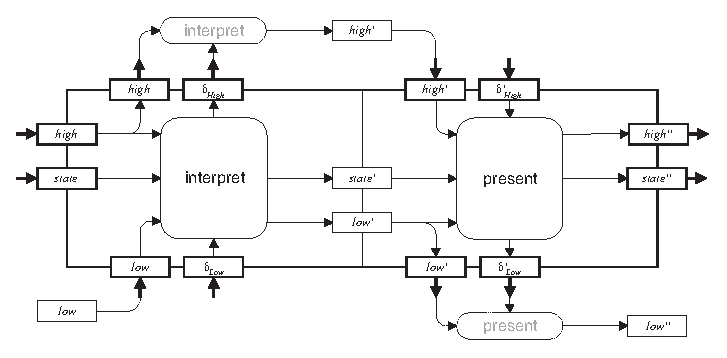
\epsfig{file=pics/eps/LayerDataFlow.eps, width=\textwidth} % visio: LayerDataFlow.vsd
\end{center}\caption{Data flow in a Proxima layer.} \label{proximaDataFlow}
\end{center}
\end{small}
\end{figure}


The data flow in the figure is encoded in the type definition for a Proxima layer. We denote the monad type constructor by \p{m} and the level types by \p{high} and \p{low}. For the edit operations (the $\delta$'s), we have distinct types for edit operations going up  (\p{editH} and \p{editL}) and edit operations going down (\p{editH'} and \p{editL'}). The reason for this distinction is that upward edit operations are often of a different nature than the downward ones.

\begin{small}
\begin{verbatim}
data Layer m state high low editH editL editH' editL' =
       Layer { interpret :: LayerFunction m (state, high) (low, editL)
                                            (state, low) (high, editH)
              , present ::   LayerFunction m (state, low) (high, editH')
                                            (state, high) (low, editL')
              }
\end{verbatim}
\end{small}

Apart from the switched directions in \p{combine} and the fact that the monadic library is used, the definitions for the Proxima architecture are virtually the same as for \p{Simple}. Moreover, the monad only affects the step type definitions and the type of the \p{lift} and \p{combine} combinators; the definitions of the combinators themselves are of the form that is described in Section~\ref{sect:libAndConclusions}. Because of the similarity, we do not reproduce the entire architecture description here.

\bc
\bigskip

The architecture combinators enforce a a strict separation between the different layers. In some cases, this . However, in general it leads to a very compositional system in which the data flow is very transparent. The addition of a new layer. Furthermore the strict separation also helped to keep user interface dependent code ... to only a few modules. Hence, adapting the system for a different user interface is not a major operation.

\bl
\o same problem as with type system. Restricting, but enforcess correctness
\o separation, all connections explicit. Very easy to add a new layer. 
\o in contrast to editors in which UI directly updates document.
\el
\ec

\bc
The motivation for using Haskell to describe editor architectures has come from the Proxima project. Proxima is a generic incremental XML editor, which is being developed at Utrecht University. The editor is parameterized with a presentation sheet that specifies how a document is presented. Furthermore, it is parameterized with a computation sheet that specifies derived values, such as chapter numbers, or a table of contents. A user can only see and edit the final presentation of the document. Because the mapping of the document on the presentation is a stepwise process, and hence the interpretation*** from edit commands on the presentation to updates on the document as well, Proxima has a layered architecture.
\ec

\bc
\begin{figure}
\begin{small}
\begin{center}
\begin{small}
\begin{tabular}{c}
{\footnotesize Document}\vspace{1ex}\\
\framebox[5cm][c]{Evaluation layer}\vspace{1ex}\\
{\footnotesize Enriched document}\vspace{1ex}\\
\framebox[5cm][c]{Presentation layer}\vspace{1ex}\\
{\footnotesize Abstract presentation}\vspace{1ex}\\
\framebox[5cm][c]{Arrangement layer}\vspace{1ex}\\
{\footnotesize Arrangement}\vspace{1ex}\\
\framebox[5cm][c]{Rendering layer}\vspace{1ex}\\
{\footnotesize Rendering}
\end{tabular}
\end{small}\caption{ The layers of Proxima}\label{proxlayers} 
\end{center}
\end{small}
\end{figure}

Figure~\ref{proxlayers} schematically shows the layers of Proxima. The figure shows the layers (surrounded by rectangles) as well as the data values that arise in the process of mapping of the document on the presentation. Edit actions and incremental updates are not shown in the figure.

The {\em document} at the top of the architecture is mapped on the {\em rendering} at the bottom, which is shown to the user. The {\em evaluator} takes the document and a computation sheet and produces the {\em enriched document}, which is the document together with all derived values. Similarly, the {\em presenter} takes the enriched document together with a presentation sheet, and computes the {\em abstract presentation}. Until this point, the presentation does not contain any absolute layout; all elements in the presentation are positioned relative to each other and do not yet have an absolute size.

The absolute coordinates are computed by the {\em arranger}. It maps the abstract presentation on an {\em arrangement}, which is a absolute positioning of all elements of the presentation. The arranger also takes care of hyphenation, line and page breaking. Finally, the arrangement is rendered to an image by the {\em renderer}.
\ec


%																
%																
%																
\section{Conclusions} \label{sect:haskellconclusions}

The combinators presented in this paper make it possible to specify layered editor architectures in a concise and transparent way. With a small number of definitions, a layered architecture can be described. The combinators have been heap profiled to ensure that no memory leaks are present, and have been used to implement the Proxima prototype as well as a database web-interface system.

Because the architecture description language is embedded in the implementation language, the architecture of a system forms part of the implementation of the system. We do not need to translate the architecture to an implementation, and hence, the implementation is guaranteed to comply with the architecture.

According to Medvidovic and Taylor~\cite{medvidovic00ADLs}, an architecture description language should describe the components of an architecture, the connectors, and the configuration. For the architecture combinators defined in this chapter, we can identify these aspects as follows: the layer functions are the components; \p{lift} and \p{combine} are the connectors; and the applications of \p{lift} and \p{combine} determine the configuration.

The combinator language in this paper is tailored to a specific kind of architectures: those of layered editors. Although we use the term editor in a broad sense, also including spreadsheets, e-mail agents, etc., further research should explore the possibilities of using Haskell to describe other kinds of architectures. Another area of research concerns how dynamic aspects of the architecture, such as the requirements of Chapter~\ref{chap:formalSpec}, can be described and, if possible, verified.

%conclusions dependent types. ?? others?
